%-*- Mode:LaTeX; -*-      
\documentclass[11pt]{article}
\usepackage{vmargin}		% Force narrower margins
\setpapersize{USletter}
\setmarginsrb{1.0in}{1.0in}{1.0in}{0.6in}{0pt}{0pt}{0pt}{0.4in}
\setlength{\parskip}{.1in}  % removed space between paragraphs
\setlength{\parindent}{0in}

\usepackage{epsfig}
\usepackage{graphicx}
\usepackage{xcolor}
\newcommand{\ra}{$\rightarrow$~}
\newcommand{\dt}{$\circ$~}

\begin{document}

\large
\begin{center}
{\bf CS-5340/6340, Written Assignment \#2} \\
{\bf DUE: Wednesday, September 22, 2021 by 11:59pm} \\ \textcolor{red}{anwsers by Jacob Herrmann u0259542}\\ ~ \\

{\bf  Submit your assignment on CANVAS in pdf format.}
\end{center}
\normalsize

\begin{enumerate}  


\item (12 pts) Consider the 9 training documents below, where each
  document consists of one sentence from (imaginary) restaurant reviews. 

\begin{center}
\begin{tabular}{|l|l|} \hline
{\bf Class} & {\bf Document} \\ \hline \hline
NEG & terrible food and slow service \\ \hline
NEG & so expensive and incredibly bad service \\ \hline
NEG & ok food but too expensive \\ \hline
NEG & service was so slow \\ \hline
POS & incredibly good food \\ \hline
POS & so tasty \\ \hline
POS & great food and not too expensive  \\ \hline
POS & service a bit slow but incredibly great food \\ \hline
POS & incredibly tasty and ok service \\ \hline
\end{tabular}
\end{center}

\hspace*{.3in}
\begin{enumerate}
\item Based on the training corpus above, compute the following
probabilities. Do not perform smoothing.  {\bf Leave your answers in
  fractional form!} 
  \textcolor{red}{negative words$=20$}
  \textcolor{red}{postive words$=24$}
  \textcolor{red}{total words$=44$}
\begin{itemize}
\item  P(NEG) 
\textcolor{red}{$=\frac{20}{44}=\frac{5}{11}$}

\item  P(POS)
\textcolor{red}{$=\frac{24}{44}=\frac{6}{11}$}

\item P(``incredibly'' $\mid$ NEG)
\textcolor{red}{$=\frac{1+4}{20+44}= \frac{5}{64}$}

\item P(``incredibly'' $\mid$ POS)
\textcolor{red}{$=\frac{3+4}{24+44}= \frac{7}{68}$}

\item P(``service'' $\mid$ NEG)
\textcolor{red}{$=\frac{3+5}{20+44}= \frac{8}{64}= \frac{1}{8}$}

\item P(``service'' $\mid$ POS)
\textcolor{red}{$==\frac{2+5}{24+44}= \frac{7}{68}$}
\end{itemize}

\hspace*{.2in}
\item Using the Naive Bayes classification algorithm, determine which
  Class (NEG or POS) would be
assigned to the test document: ``incredibly expensive but ok''. 
{\bf Show ALL of your work! You will get zero credit if you only give
  a class name without showing the work.}


\end{enumerate}
\begin {enumerate}
  \color{red}
  \item[] Class Priors
   \\* \quad $P(-)=\frac{4}{9}$ \quad $P(+)=\frac{5}{9}$
   \item[] Sample Likelihood probs
   \\* \quad $P(``incredibly'' \mid-)=\frac{5}{64}$ \quad $P(``incredibly'' \mid+)=\frac{7}{68}$
   \\* \quad $P(``expensive'' \mid-)=\frac{5}{64}$ \quad $P(``expensive'' \mid+)=\frac{4}{68}$
   \\* \quad $P(``but'' \mid-)=\frac{3}{64}$ \quad \quad\quad \quad $P(``but'' \mid+)=\frac{3}{68}$
   \\* \quad $P(``ok'' \mid-)=\frac{3}{64}$ \quad \quad  \quad\quad$P(``ok'' \mid+)=\frac{3}{68}$
  \item[] Test ``incredibly expensive but ok''
  \\* \quad $P(-)P(S\mid-)= \frac{5}{11}* \frac{5*5*3*3}{64^4}=6.0959E-6$
  \\* \quad $P(+)P(S\mid+)= \frac{6}{11}* \frac{7*4*3*3}{68^4}=6.4287E-6$
  \item [] POS
\end{enumerate}

\newpage
\item (26 pts) Use the following tables of probabilities 
to answer this question. Note that these numbers are 
fictional and do not necessarily add up logically (i.e., sum to 1
where they should), but don't worry about that, just use them as they
are.  There are only 2 possible part-of-speech tags: N (noun) and V (verb). 

\begin{center}
\begin{tabular}{|lr|} \hline
P(police $\mid$ N) & .60 \\ \hline
P(police $\mid$ V) & .20 \\ \hline
P(tax $\mid$ N) & .50 \\ \hline
P(tax $\mid$ V) & .40 \\ \hline
P(returns $\mid$ N) & .30 \\ \hline
P(returns $\mid$ V) & . 10 \\ \hline
\end{tabular}
\hspace*{.5in}
\begin{tabular}{|lr|} \hline
P(N $\mid$ $\phi$) & .85 \\ \hline
P(V $\mid$ $\phi$) & .15 \\ \hline
P(N $\mid$ N) & .65 \\ \hline
P(N $\mid$ V) & .55 \\ \hline
P(V $\mid$ N) & .45 \\ \hline
P(V $\mid$ V) & .25 \\ \hline
\end{tabular}
\end{center}

The following network would be used by the Viterbi algorithm
to find the most likely sequence of POS tags for the sentence {\it
  ``Police tax returns''}: 

\begin{center}
\psfig{figure=viterbi-pic.png,height=1.2in}
\end{center}

\begin {enumerate}
  \color{red}
  \item[] Police 
  \\* \quad  $ P(Police\mid N)*P(N\mid\phi)=0.60 * .85= 0.51$
  \\* \quad  $ P(Police\mid V)*P(V\mid\phi)=0.20 * .15= 0.03$
  \item[] tax
  \\* \quad  $ P(tax\mid N)*Max[P(N \mid N),P(N \mid V)]=0.50 *Max[0.65,0.55]= 0.325$
  \\* \quad  $ =0.325*0.51= 0.16575$
  \\* \quad  $ P(tax\mid V)*Max[P(V \mid N),P(V \mid V)]=0.40 *Max[0.45,0.25]= 0.18$
  \\* \quad  $ =0.18*0.51 =0.0918$

  \item[] returns
  \\* \quad  $ P(return\mid N)*Max[P(N \mid N),P(N \mid V)]=0.30 *Max[0.65,0.55]= 0.195$
  \\* \quad  $ =0.195*0.16575= 0.03232$
  \\* \quad  $ P(return\mid V)*Max[P(V \mid N),P(V \mid V)]=0.10 *Max[0.45,0.25]= 0.045$
  \\* \quad  $ =0.045*0.16575= 0.00745$
  \item[] best tag path is N N N with 0.03232

\end{enumerate}

\newpage

\begin{enumerate}
\item Using the Viterbi algorithm, compute the probability for each of the
following nodes in the network. Show all your work! \\

\begin{itemize}

\item P(police=N)  \\
\textcolor{red}{\quad  $ P(Police\mid N)*P(N\mid\phi)=0.60 * .85= 0.51$}
\item P(police=V)  \\
\textcolor{red}{\quad  $ P(Police\mid V)*P(V\mid\phi)=0.20 * .15= 0.03$}
\item P(tax=N) \\
\textcolor{red}{\quad  $ P(tax\mid N)*Max[P(N \mid N),P(N \mid V)]=0.50 *Max[0.65,0.55]= 0.325$}
\item P(tax=V) \\
\textcolor{red}{\quad  $ P(tax\mid V)*Max[P(V \mid N),P(V \mid V)]=0.40 *Max[0.45,0.25]= 0.18$}
\item P(returns=N) \\
\textcolor{red}{ \quad  $ P(return\mid N)*Max[P(N \mid N),P(N \mid V)]=0.30 *Max[0.65,0.55]= 0.195$}
\item P(returns=V) \\
\textcolor{red}{\quad  $ P(return\mid V)*Max[P(V \mid N),P(V \mid V)]=0.10 *Max[0.45,0.25]= 0.045$}
\end{itemize}


\newpage
\item Compute the following forward probabilities.  Show all your work! \\

\begin{itemize}


\item $\alpha_{tax}(N)$ \\
\textcolor{red}{\quad  $=P(tax\mid N)*SUM[P(N \mid N),P(N \mid V)]=0.50 *SUM[0.65,0.55]= 0.6$}

\item $\alpha_{tax}(V)$ \\
\textcolor{red}{\quad  $=P(tax\mid V)*SUM[P(V \mid N),P(V \mid V)]=0.40 *SUM[0.45,0.25]= 0.28$}


\end{itemize}


\item Compute the following normalized probability values. Show all  your work! \\

\begin{itemize}

\item P(tax/N  $\mid$ police) \\
\textcolor{red}{\quad  $=\frac{\alpha_{police}(N)}{\sum\alpha}=\frac{0.51}{SUM[0.65,0.55]}= 0.425$}

\item P(tax/V  $\mid$ police) \\
\textcolor{red}{\quad  $=\frac{\alpha_{police}(V)}{\sum\alpha}=\frac{0.03}{SUM[0.45,0.25]}= 0.0428$}

\end{itemize}


\end{enumerate}



\newpage
\item (28 pts) Assume that a part-of-speech (POS) tagger has been applied to the
sentence below with the following results:

\begin{quote}
{\bf Bob}/{\sc noun~} {\bf put}/{\sc verb~} {\bf the}/{\sc art~} {\bf
  light}/{\sc adj~} {\bf blue}/{\sc adj~}
{\bf light}/{\sc noun~}  {\bf bulb}/{\sc noun~} {\bf in}/{\sc prep~} \\
{\bf the}/{\sc art~}  {\bf blue}/{\sc adj~}   {\bf light}/{\sc noun~}  {\bf fixture}/{\sc noun~}  
{\bf to}/{\sc inf~} {\bf light}/{\sc verb~} 
{\bf the}/{\sc art~} \\ {\bf orange}/{\sc adj~} 
  {\bf and}/{\sc conj~} {\bf blue}/{\sc adj~}  {\bf room}/{\sc noun~} 
{\bf with}/{\sc prep~} {\bf brilliant}/{\sc adj~} {\bf light}/{\sc
  adj~} \\
{\bf blue}/{\sc adj~} {\bf light}/{\sc noun~} {\bf !}/{\sc punc}
\end{quote}
\vspace*{.1in}

We define the various types of probabilities as follows, where $w_i$
indicates a word and $t_i$ indicates a POS tag. 

\begin{itemize}
\item $P(w_i)$ means probability of word $w_i$
\item $P(w_i~w_j)$ means probability of the bigram $w_i$ $w_j$ . Do
  not use $\phi$  as a part of any bigrams. 
\item $P(t_i)$ means probability of POS tag $t_i$
\item $P(t_i~t_j)$ means probability of the bigram $t_i$ $t_j$ . Do
  not use $\phi$ as a part of any bigrams. 
\item $P(w_i \mid w_{i-1})$ means probability of word   $w_i$   following word $w_{i-1}$
\item$P(w_i \mid w_{i-2}~w_{i-1})$ means probability of word $w_i$  following words $w_{i-2}$ $w_{i-1}$ 
\item$P(t_i \mid t_{i-1})$ means probability of POS  tag $t_i$ following POS tag $t_{i-1}$
\item$P(t_i \mid t_{i-2}~t_{i-1})$ means probability of word $t_i$ following words $t_{i-2}$ $t_{i-1}$
\item$P(w_i \mid t_i)$ means  probability of word $w_i$ given tag $t_i$.
\item$P(t_i \mid w_i)$ means  probability of tag $t_i$ given word $w_i$.
\end{itemize}

Fill in the table below with the probabilities that you would estimate
based on the tagged sentence above. {\bf Leave your results in fractional
  form (e.g., 5/5)!}  If a probability would be undefined (i.e.,
have a zero denominator), then answer UNDEFINED. 

  \begin{center}
  \begin{tabular}{|l|l|} \hline
  \textbf{Probability~~~~~~~~~~~~~~~} & \textbf{Value~~~~~~~~~~~~~~~~~} \\ \hline
  $P$(blue) &  \textcolor{red}{$\frac{4}{25}$}\\ \hline
  $P$(to light) & \quad \textcolor{red}{$\frac{1}{25}$}\\ \hline
  $P$(ADJ) & \textcolor{red}{$\frac{8}{25}$}\\ \hline
 $P$(NOUN NOUN) & \quad \textcolor{red}{$\frac{2}{25}$}\\ \hline
  $P$(blue $\mid$ light) & \textcolor{red}{$\frac{2}{6}$}\\ \hline
  $P$(light $\mid$ to) & \quad \textcolor{red}{$\frac{1}{1}$}\\ \hline
 $P$(bulb $\mid$ blue light) & \textcolor{red}{$\frac{1}{3}$} \\ \hline
  $P$(VERB $\mid$ NOUN) & \quad \textcolor{red}{$\frac{1}{7}$}\\ \hline
  $P$(ADJ $\mid$ ADJ) & \textcolor{red}{$\frac{3}{8}$}\\ \hline
  $P$(NOUN $\mid$ ART ADJ) & \quad \textcolor{red}{$\frac{3}{8}$} \\ \hline
  $P$(blue $\mid$ ADJ) & \textcolor{red}{$\frac{2}{8}$}  \\  \hline
  $P$(light $\mid$ NOUN) & \quad \textcolor{red}{$\frac{0}{7}$} \\ \hline
  $P$(NOUN $\mid$ Bob) & \textcolor{red}{$\frac{0}{1}$}  \\ \hline
  $P$(VERB $\mid$ light) & \quad \textcolor{red}{$\frac{0}{6}$}  \\ \hline
  \end{tabular}
  \end{center}


\newpage

\newpage
\item (16 pts) Consider the following four context-free grammars that
  recognize Noun Phrases (NPs). Assume that you want to find grammar
  derivations beginning with the non-terminal ``NP''. 

\begin{center}
\begin{tabular}{|l|l|l|l|} \hline
{\bf G1} & {\bf G2} & {\bf G3} & {\bf G4} \\ \hline
NP \ra art NP1   & NP \ra art X    & NP \ra NP7         & NP \ra art W \\
NP \ra NP1       & NP \ra adj X    & NP \ra art NP6     & NP \ra W \\
NP1 \ra adj NP1  & NP \ra X        & NP \ra adj NP6     & W \ra adj noun \\
NP1 \ra NP2      & X \ra adj Y                & NP \ra art adj NP6 & W \ra adj W \\
NP2 \ra noun     & Y \ra noun      & NP6 \ra NP7        & W \ra Z \\
NP2 \ra noun NP2 & Y \ra noun noun      & NP7 \ra noun NP7   & Z \ra noun Z \\
~                & Y \ra noun Y & NP7 \ra noun       & Z \ra noun \\ \hline
\end{tabular}
\end{center}

For each pair of grammars below, give an example of a sequence of
part-of-speech (POS) tags that would be recognized as a legal NP by
the first grammar but not the second grammar. If there is no such tag sequence
then answer {\it No Sequence}.

\begin{enumerate}

\item  list a tag sequence recognized by G1 but not G2
\textcolor{red}{NP\ra NP1 \ra NP2}
\item list a tag sequence recognized by G2 but not G1
\textcolor{red}{NP\ra adj X}
\item list a tag sequence recognized by G1 but not G3
\textcolor{red}{NP\ra NP1 \ra adj NP1 }
\item list a tag sequence recognized by G3 but not G1
\textcolor{red}{NP \ra art adj NP6 }
\item list a tag sequence recognized by G1 but not G4
\textcolor{red}{no sequence}
\item list a tag sequence recognized by G4 but not G1
\textcolor{red}{NP \ra W \ra adj noun }
\item list a tag sequence recognized by G2 but not G3
\textcolor{red}{NP \ra X \ra Y \ra noun noun }
\item list a tag sequence recognized by G3 but not G2
\textcolor{red}{NP \ra art adj NP6 }

\end{enumerate}

\newpage
\item (12 pts) Pretend that the parse trees below are a (tiny!) parsed text
  corpus. Fill in the table below with all of the context-free grammar
  rules that appear in   these parse trees and the total frequency
  count of each rule. For example, if the same grammar rule appears
  twice in one parse tree and once in the other parse tree, then its
  frequency count should be 3. 

\begin{center}
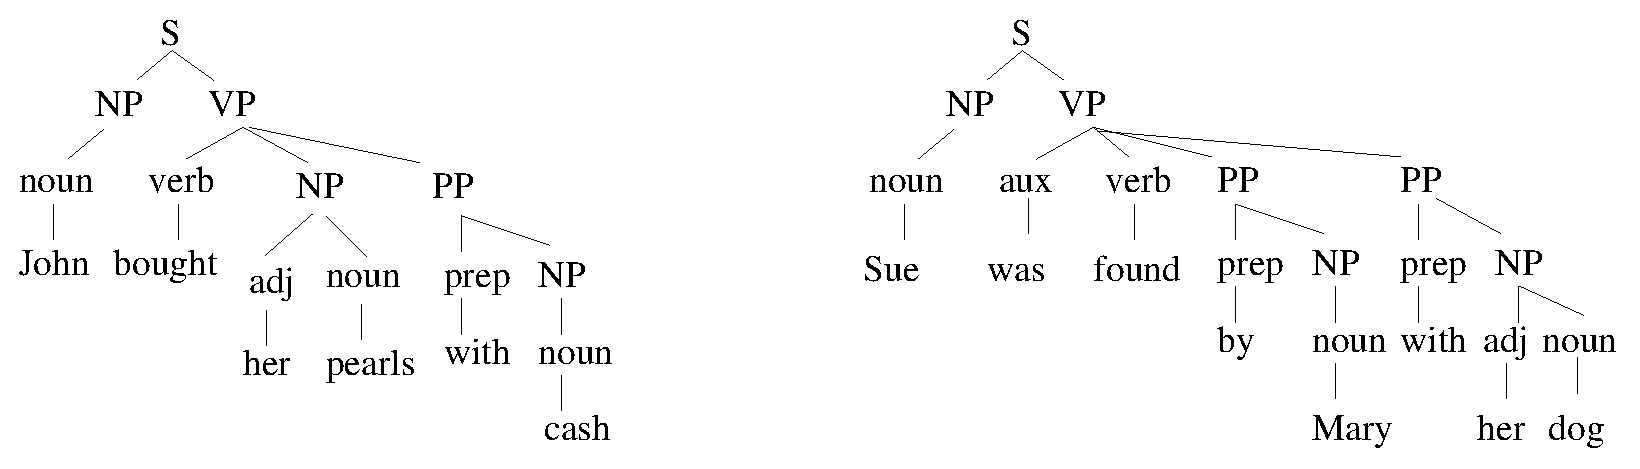
\includegraphics[width=6.5in]{trees1.eps}
\end{center}

 \vspace*{.1in}
 \begin{center}
 \begin{tabular}{|l|c|}  \hline
 \textbf{Grammar Rule} & \textbf{Frequency} \\ \hline
 \textcolor{red}{S \ra NP VP}& \textcolor{red}{2} \\
 \textcolor{red}{NP \ra noun} & \textcolor{red}{4} \\
 \textcolor{red}{VP \ra verb NP PP} & \textcolor{red}{1}  \\
 \textcolor{red}{NP \ra adj noun} & \textcolor{red}{2}\\
 \textcolor{red}{PP \ra prep NP}& \textcolor{red}{3} \\
 \textcolor{red}{VP \ra aux verb PP PP} & \textcolor{red}{1} \\
~ & ~ \\
~ & ~ \\
~ & ~ \\
~ & ~ \\
~ & ~ \\
~ & ~ \\
~ & ~ \\
~ & ~ \\
~ & ~ \\
~ & ~ \\
~ & ~ \\
~ & ~ \\
~ & ~ \\
~ & ~ \\ \hline
 \end{tabular}
 \end{center}



\newpage
\item (6 pts) Consider the grammar below:

\begin{center}
\begin{tabular}{|ll|} \hline
\textbf{Grammar Rules} & \\  \hline
S $\rightarrow$ NP VP & noun $\rightarrow$ {\it NLP} \\
NP $\rightarrow$ noun & verb $\rightarrow$ {\it is} \\
VP $\rightarrow$ verb & adj $\rightarrow$  {\it cool} \\
VP $\rightarrow$ verb ADJP & ~ \\
ADJP $\rightarrow$ adj & ~ \\ \hline
\end{tabular}
\end{center}

Show a bottom-up, depth-first search derivation of the parse for the
  sentence {\it ``NLP is cool''} using the grammar above. Search the grammar based on
  the order of the rules in the table above (i.e., apply the ``VP $\rightarrow$
   verb'' rule before the other VP rule). 
Do NOT use chart parsing -- just show a generic search-based derivation!
\\
\begin{enumerate}
  \color{red}
  \item[]  NLP is cool
  \item[]  {\it noun} is cool
  \item[]  {\it NP} is cool
  \item[]  {\it NP verb} cool
  \item[]  {\it NP VP} cool
  \item[]  {\it S} cool
  \item[]  {\it NP verb} cool
  \item[]  {\it NP verb adj} 
  \item[]  {\it NP verb ADJP} 
  \item[]  {\it NP VP} 
  \item[]  {\it S} 
\end{enumerate}

\newpage
\underline{\textbf{Question \#7 is for CS-6340 students ONLY!}}  \\

\item (24 pts) Consider the grammar G below:

\begin{center}
\begin{tabular}{|ll|} \hline
\textbf{Grammar} & ~ \\  
S $\rightarrow$ NP VP    & NOUN \ra John \\
S $\rightarrow$ VP NP    & NOUN \ra can \\
NP $\rightarrow$ NOUN    & NOUN \ra well \\
VP $\rightarrow$ MOD VP1 & VERB \ra swim \\
VP1 $\rightarrow$ VERB   & MOD \ra can \\
VP1 $\rightarrow$ VERB ADV & ADV \ra well \\  \hline
\end{tabular}
\end{center}

List all of the entries that would be put on the chart by the {\it Earley
chart parsing algorithm} when parsing the sentence {\bf ``John can swim
  well''}.  Each chart entry should be a constituent or a rule, with a
start and end position indicating which words have been matched by the
constituent or rule. Assume that {\bf ``John''} is in position 1 and
{\bf ``well''} is in position 4.

To get you started, the list below contains the chart entries for all
of the part-of-speech tag constituents. Your job is to complete
this list by adding the rest of the constituents and rules that would
be added to the chart during parsing.

When a rule is added to the chart,  use an asterisk (*) to separate the components
of the rule that have been matched from the ones that have not yet
been matched. For example, the rule: \\ {\bf S $\rightarrow$ * NP VP
  [1-1]} means that nothing in this rule has been matched yet but
the rule can begin matching constituents starting in position 1.  The
rule {\bf S $\rightarrow$ NP * VP [1-2]} means that the NP has
successfully matched words in the span [1-2] and the rule is waiting to match a VP
starting in position 2.

\newpage
\begin{center}
{\bf CHART ENTRIES FOR ``John can swim well''}  \\ ~ \\

 \begin{tabular}{lc} 
 {\bf Constituent or Rule~~~} & {\bf ~~~Start-End} \\ \hline
 NOUN(``John'') &  [1-2] \\
 NOUN(``can'') & [1-2] \\
 MOD(``can'') & [2-3] \\
 VERB(``swim'') & [3-4] \\
 NOUN(``well'') & [4-5] \\
 ADV(``well'') & [4-5] \\
 ~ & ~ \\
 \textcolor{red}{S \ra * NP VP} & \textcolor{red}{[1-2]}\\
 \textcolor{red}{NP \ra * NOUN} & \textcolor{red}{[1-2]}\\
 \textcolor{red}{NOUN \ra NOUN(``John'')} & \textcolor{red}{[1-2]}\\
 \textcolor{red}{NP} & \textcolor{red}{[1-2]}\\
 \textcolor{red}{S \ra NP * VP} & \textcolor{red}{[1-3]}\\
 \textcolor{red}{VP \ra *MOD VP1} & \textcolor{red}{[2-3]}\\
 \textcolor{red}{MOD \ra  MOD(``can'')} & \textcolor{red}{[2-3]}\\
 \textcolor{red}{VP \ra MOD * VP1} & \textcolor{red}{[2-4]}\\
 \textcolor{red}{VP1 \ra VERB} & \textcolor{red}{[3-4]}\\
 \textcolor{red}{VERB \ra VERB(``swim'')} & \textcolor{red}{[3-4]}\\
 \textcolor{red}{VP1} & \textcolor{red}{[3-4]}\\
 \textcolor{red}{VP} & \textcolor{red}{[2-4]}\\
 \textcolor{red}{S \ra NP VP *} & \textcolor{red}{[1-4]}\\
 \textcolor{red}{S} & \textcolor{red}{[1-4]}\\
 \textcolor{red}{VP1 \ra VERB * ADV} & \textcolor{red}{[3-5]}\\
 \textcolor{red}{ADV \ra ADV(``well'')} & \textcolor{red}{[4-5]}\\
 \textcolor{red}{VP1} & \textcolor{red}{[3-5]}\\
 \textcolor{red}{VP} & \textcolor{red}{[2-5]}\\
 \textcolor{red}{S \ra NP VP *} & \textcolor{red}{[1-5]}\\
 \textcolor{red}{S} & \textcolor{red}{[1-5]}\\
 \textcolor{red}{S \ra * VP NP} & \textcolor{red}{[1-2]}\\
 \textcolor{red}{VP \ra *MOD VP1} & \textcolor{red}{[1-2]}\\
 \end{tabular}
 \end{center}



\end{enumerate}

\end{document}
